\documentclass[11pt,twoside,a4paper]{article}
\usepackage{mathptmx}
\usepackage{marvosym}
\usepackage[english]{babel}
\usepackage{graphicx}
\usepackage{parskip}
\usepackage{fancyvrb,url}
\usepackage{amsmath}
 
\begin{document}
\title{Language Independent Dependently Typed Core}
 \author{Tamar Christina\\
 Dept. Information and Computing Science,\\
 Utrecht University,\\
 Research Proposal (Pre-Draft) \\
 \texttt{T.Christina@students.uu.nl}}
 \date{\today}
 \maketitle

\section{Motivation}
Every year hundreds of thousands if not millions are spend in testing programs for correctness, more are spend on creating the Tests themselves and the people to run these tests. Projects are routinely late because of programming errors. In computer science programming errors are referred to as Bugs. They not only indicate a program crash, but also any behavior of a program of function which is not specified or conforming to a predetermined specification. These errors cost more the later they are found in the development lifecycle\cite{code}, in fact an error that costs \EUR{1000},- during the programming phase can cost \EUR{5000},- during the testing phase.  Other errors depending on how early they are caught can end up costing up to 25x times the amount it would have to fix early on.

It doesn't help that programs are increasingly becoming more complex and the time allotted to develop them is becoming shorter all around. This creates an increasingly large pressure to get things right the first time around. That is where type systems come in. A type system provides a means of determining the absence of certain kind of programming errors at compile time. The compiler would reject these programs instead of allowing them to be created and then subsequently shipped without the being detected.  A type system enforces a contract between a caller and its arguments. An example of this is that if you would try to evaluate 1 / "hello" the compiler would reject such a program, stating the fact that "hello" is not a number, and since the division operator / requires two numbers this program is considered ill-typed and is this rejected. 

A characterization of a type system is: \begin{quote}
"A Type system is a tractable syntactic method for proving the absence of certain program behaviors by classifying phrases according to the kinds of values they compute"\cite{pierce}
\end{quote}

This definition implies that type systems are a form of formal correctness prover, they provide a number of important functions namely:

\begin{description}
\item[Safety] Rejecting of ill-typed programs at compile time, catching bugs sooner rather than later thus saving time and money.
\item[Optimization] Because types are known at compile time, more efficient code can be generated making programs that run faster.
\item[Documentation] The more expressive the type system, the more it says about the function and how to use it and which values to express as a result. This serves as part of the documentation as to the meaning of the function.
\item[Abstraction] They allow programmers to think of programs from a much higher level, without worrying about how a particular data structure has been implemented.
\end{description}

Not all type systems are created equally however. Programming languages like Haskell\cite{Haskell} provide very strong type systems compared to languages such as C and C++. Even though errors can be caught much earlier on using Haskell than using lower level languages such as C or C++, Haskell programs tend to be slower than their imperative counterparts\cite{benchmark}.

Most recently a lot of research is being done on dependently typed programming languages. Languages such as Coq\cite{Coq} and Agda\cite{Agda} are becoming increasingly popular because of their ability to statically(at the time of compilation) check for more incorrect behavior of a program compared to other programming languages. Because dependently typed type systems are also proof assistants they also provide you with a proof of correctness. Consider the type of the matrix multiplication function: 

\begin{equation}
matrix\_multiply : matrix_{(k,m)} \times matrix_{(m,n)} \rightarrow matrix_{(k,n)}
\end{equation}

It says that the inputs should be matrices, one of size (k,m) the other (m, n) and that the output of invoking the function on two valid arguments will be a matrix of size (k,n).  Not only are the types of the checked but also a depend property on the types, namely the size of the matrices. In order to define such a function you need to be able to provide sufficient evidence to the type system to satisfy the constraints on the types. 

This flexibility allows it to find more kinds of errors without even having to run the program, which means bugs are caught early on saving money and valuable resources. Not only that but less tests should be written to test the program because we already have a proof of correctness.

Sadly, dependently typed programming languages are not as main stream as Java or C++ even though they provide much better quality control and static checking abilities. This is in my opinion due to that they are usually harder to use and learn and the programs they produce are generally slower than those produced by the competing languages. For these two reasons they are often not used even though they provide a higher degree of safety.
\section{Research}
\emph{I propose the construction of an intermediate dependently typed Core language that other programming languages can translate to as a backend. Which will provide the same level of Safety as is to be expected from a dependently typed language, but to also use this extra typing information to produce applications that perform competitively.}

\section{Approach}
Along the way to completing the task at hand there are a few milestones, each can stand on its own but they ultimately form a whole.

\subsection{Core language development}
The first component that needs to be created is the actual language, taking as inspiration TyCore \cite{super} and GHC Core \cite{pierce}. First a complete specification has to be made. This includes developing both Syntax and Semantics. 

Being a dependently typed core language means that it will also have lifted values to the domain of types. The difficulty here is trying to come up with a language that's complete enough to be able to describe rich languages such as Agda and Haskell, but also one that we can gain the most opportunities for optimizations from. 

One way to do it is to limit as much as possible the amount of expression that are supported in the language while not limiting its expressiveness.  This would also make it easier to perform type checking in the language itself in case that has not been done. Since we need to have typing information, it's a good idea to also develop a type system for the language, or at least adapt an existing type system to the core language being developed.
\subsection{Strictness Analyzer}
In order to perform certain kinds of optimization in order to make the code generated perform competitively a strictness analyzer has to be developed for the language and its constructs. 

A strictness analyzer looks at the arguments of a function and determines whether they are strict or non-strict. In terms of higher-order functions this is especially tricky. 
This is not a trivial task. 

\subsection{Supercompilation on Core language}
One of the most important parts of making a competitive language from a higher level language is how we can speed up the execution time of the application. One way to do this is to evaluate as much as possible at compile time. This means simplification and evaluation rules should be developed for the language. They have to be proven safe and in the end will have an added side effect of creating more optimization opportunities.

\subsection{Calling convention \& other optimizations}
With the strictness analyzer in place and a simplified AST, the next thing to look at is what other optimizations we can apply.  Calling convention optimizations is one we can certainly apply. But having a fully developed language means that we can find more opportunity for optimizations.

\subsection{Embedding in UHC}
In order to evaluate the practicality and real world performance of the backend an implementation for UHC will be provided.  UHC is the Utrecht Haskell Compiler which is a collection of smaller compilers. This makes it ideal for experimentation since different parts of it can be implemented independently of each other. To illustrate where in the pipeline of UHC this would fit in the makeup of UHC should be explained:

\begin{figure}[h!]
  \centering
    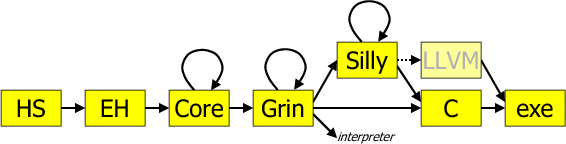
\includegraphics[width=0.8\textwidth]{UHC}
  \caption{UHC pipeline}
\end{figure}

The front-end of the UHC compiler reads in Haskell code and converts it to EH \emph{(Essential Haskell)} code. \emph{Essential Haskell} is a de-sugared form of Haskell. The bindings are also arranged in a manner that most actions like type checking can be done in a single top-down pass. 

Every compiler performs the first two stages. The first part, the parser converts the \emph{concrete syntax} (e.g. what the user writes down) into \emph{abstract syntax} (what the compiler uses and what the code actually means). After this phase the \emph{abstract syntax} is de-sugared and converted into the internal representation that the compiler will continue using. De-sugaring is needed because programming languages provide a lot of convenience syntax for programmers. They make things easier to understand for programmers but they're not needed in terms of the core syntax of the language.

The next three phases: Core, Grin, Silly are all different optimization phases. They each have their own syntax and optimization passes. The optimizations get increasingly low level the deeper in the pipeline you go. 
The next blocks are code generation blocks, where an actual executable gets generated. TyCore would fit into the pipeline as follows.

\begin{figure}[h!]
  \centering
    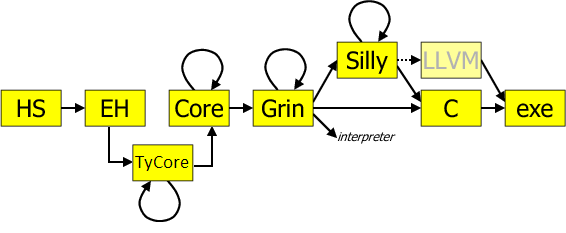
\includegraphics[width=0.8\textwidth]{UHC-TyCore}
  \caption{UHC pipeline}
\end{figure}

\subsection{Evalutaiton \& Benchmarks}
At the end, to prove that the results are what were claimed, I will provide benchmarks on the "classical" UHC and the one with the developed backend. In order to prove that the language can also optimize other languages we will provide a frontend for another language and compare its results as well.

\section{Related work}
\subsection{Types are calling conventions\cite{types}}
In this paper Maximilian C. Bolingbroke and Simon Peyton Jones introduce an idea that we can use the arguments of functions themselves as a sort of calling convention. A calling convention describes among other things how arguments should be passed to a function, what to expect as the result of applying a function to some or all arguments, how many arguments should be given to the function etc.

In terms of lazy languages such as Haskell an interesting is how laziness is achieved, if a function always evaluated an expression, it should be possible to instead of passing a thunk to the function that we evaluate it and pass the actual value. This saves us the overhead of passing thunks, and in some instances, of even creating them.

A core language for Haskell is introduced that is based on A-normal form. It is an explicitly typed language\footnote{Explicitly typed means that for every value, terms and expression a type has been given} which is similar to SystemF but with a slightly more expressive type scheme so that calling conventions can be expressed. It is used in part as inspiration to the next topic.

\subsection{Strictness Optimization in a Typed Intermediate Language\cite{Tom}}
In this thesis project Tom Lokhorst has demonstrated that a dependently typed core language can be used for optimizations. It is based on the External GHC core, Henk and strict\footnote{This means arguments are passed by value (e.g. no thunking)} Core.  It is also an explicitly typed Strict language . It supports the passing of multiple arguments at once and the returning of multiple arguments at once from a function. It also has a single representation for values, types and kinds. Kinds are the types of Types. Just as every value has a type, every type also has a type.

To illustrate this, the identity function id is defined as
\begin{align*}
Id : <a:_1*> \hspace{5pt} \rightarrow  \hspace{5pt}  <\_:a> \hspace{5pt} \rightarrow \hspace{5pt} <\_:a> \\
 = \lambda<a:_1*> <x:a> \hspace{5pt} \rightarrow \hspace{5pt} <x>
\end{align*}

Because the same syntax is used for both terms and types, the $:_1$ is used to indicate that we're talking about a value. The type of the function about reads as "for a type a with kind *, the function id takes an argument of type a and returns a value of type a" the $<$$>$ are used to indicate sequences of values. This is how multiple arguments are passed or received.

As the function above demonstrates the types of an argument are also part of the function itself. Which means that when applying the function one of the arguments should be a type argument. An example is id $<$Int$>$ $<$3$>$.

Even though TyCore is strict it can still express laziness. This is done by having explicit notation for laziness which is denoted using \{\}. For instance $<$\{Int\}$>$ means a lazy sequence. In order to force a lazy computation the notation $\|\|$ is used. E.g. $\|x\|$ forces the computation of x.

The most obvious and simplest optimization that can be done is Arity raising. This in effect is just combining multiple arguments from a function into one longer sequence. This is not always possible and should be done with care.

The second optimization is strictness optimization. This is a rather tricky bit, and the more expressive the core language the more difficult this becomes. As mentioned before one important thing is to if possible pass values strictly when possible. This saves memory and time. One might be inclined to ask themselves why we don't always pass an argument strict. The reason for that is that Haskell (and a few other languages) is a lazy language. Passing all arguments as strict would change the semantics of the language and produce erroneous results. To illustrate this consider the function const. Const takes two values and just returns the 1st value and discards the second one. In a lazy language const 1 (2/0) would succeed returning 1. But if we were to pass every argument strictly then before const is even called we would get a division by 0 exception due to the evaluation of the second argument.

In order to achieve strictness optimization every argument is annotated with an annotation indicating whether it's strict or not. An argument is strict in a function if it is inspected inside the body of the function.  In most functional languages functions are first class citizens, which means we can pass functions as arguments to functions and receive functions as a result of a computation.

If we were to look at the function map :: $(a \rightarrow b) \rightarrow [a] \rightarrow [b]$, which maps a function from \emph{a} to \emph{b} on every element of a list of \emph{a}'s returning a list of \emph{b}'s. Determining whether the arguments of the function passes to map is strict or lazy depends on the function that is passed to map. For instance passing (+1) to map indicates that \emph{a} is strict, while if we pass (const 1) then \emph{a} is lazy.

\subsection{A Supercompiler for Core Haskell}
This paper by Neil Mitchell and Colin Runciman \cite{super} introduces the concept of supercompilation on a Haskell core language. The concept of supercompilation entails evaluating the program as much as possible at the time of compilation. The idea being that after doing this the resulting residual program would be more efficient and execute faster because it has less work to do compared to the starting program.

It attacks the problem on 3 fronts:

\begin{description}
\item[Deforestation]{ During a long chain of computations, especially with lists, intermediate values are produced and consumed at ever link in the chain as it calculates the results. This is an obvious source of inefficiency as memory has to be reserved, written to and read from for each of these intermediate lists. The idea of deforestation is to change the program in such a way that no intermediate lists are created or needed.

This would speed up computation such as "print . length . words =$<$$<$ getContents" where without this optimization first the content is read in and put in a list, then this lists is split up into lists of lists, then the length is calculated by traversing this list again and finally we can print the length.
}
\item[Argument passing]{ Functions are first class citizens in functional programming languages. This offers a great amount of flexibility and abstraction but also introduces a source of inefficiency. Consider the function \emph{dropWhile} that expects as a first argument a function which acts as a predicate and determines whether to stop dropping values from the list. 
This function is written recursively; in each iteration it calls itself passing the same function as an argument. Having to continually pass this argument along is a pretty expensive thing.
}
\item[Thunks]{ In lazy languages computations are performed as needed. This enabled the ability to defer computing something to a later time. In order to do this there needs to be a way to express and store suspended computations. Such suspended computations are called Thunks. When a thunk is forced its value is computed and the thunk is then updated with this value. Creating a thunk is not a cheap operation, it costs time and resourced. If we think back to deforestation and argument passing it now becomes clear that having to create intermediate lists or repeatedly passing the same argument around is quite expensive.  This is handled in this paper by creating specialized functions which have been partially applied to some of its arguments.}
\end{description}

The main contributions of this paper are a reasonable stopping criteria for the unfolding of definitions and a strategy for evaluation. They focus all their optimization strategies on only \emph{case} expressions and \emph{Let} bindings.

They go about by it defining a Split function that given an expression returns the expression with \emph{holes} in them and a list of child expressions which were in the place of these holes. They then try to optimize the child expressions and then the parent expression as a whole, having filled in the holes.

What's been shown is that a dependently typed core language is both feasible and practical for optimization needs.  However it stops short of defining a complete formal syntax and semantics for such a language. It proves what can be done, but just scratches the surface on the possibilities.

\section{Expected contibutions}
None of the examples above form a cohesive whole, and most of them stop short of giving a practical specification. They all prove that some parts of what's proposed here is possible, at least to a very specific language.

The contributions I intend to make in this field are:

\begin{description}
 \item[Provide a language agnostic strongly typed core language] \hfill \\
 A core language that can potentially be used in individual compilers as a backend to perform various transformations or optimizations on. Such a language would help further the adoption of dependently typed languages by giving a common language which all compiler writers can work on improving. \cite{Tom}
 \item[Specify and develop a set of optimizations to improve performance] \hfill \\
A set of optimizations to make it possible to generate more efficient code and provide better resource management \cite{types}
 \item[Provide type safe program transformations] \hfill \\
A collection of static program transformations to evaluate as much as possible at compile time. And to expose more potential points of optimizations. Based on Supercompilation \cite{super}
 \item[Provide an example implementation in the Utrecht Haskell Compiler] \hfill  \\
To illustrate that the language is capable of all that's claimed a reference implementation will be provided for the Utrecht Haskell Compiler, along with benchmarks comparing the different compiler/languages.
 \end{description}
\begin{thebibliography}{9}
\bibitem{code}
  McConnell, Steve
  \emph{ Code Complete. 1st}
  Redmond, Washington : Microsoft Press, 1993. pp. 25-26. ISBN 1-55615-484-4.
\bibitem{benchmark}
  Computer Language Benchmark. [Online] 2010. [Cited: November 24, 2010.] \url{http://shootout.alioth.debian.org/u32q/benchmark.php?test=all&lang=ghc&lang2=gcc}
\bibitem{super}
  Mitchell, Neil and Runciman, Colin.
  \emph{A Supercompiler for Core Haskell}
  2008, IFL, pp. 147-164.
\bibitem{Tom}
  Lokhorst, Tom. 
  \emph{Strictness Optimization in a Typed Intermediate Language.}
   Utrecht, The Netherlands : Dept. of Information and Computing Sciences, 2010.
\bibitem{types}
  Bolingbroke, Maximilian C. and Jones, Simon L. Peyton.
  \emph{Types Are Calling Conventions.} 
  2009, ACM.
\bibitem{pierce}
  Benjamin C. Pierce and David N. Turner
  \emph{Local Type Inference}
  Indiana University and Technology Transfer Center
\bibitem{Haskell}
	A purely functional programming language \url{Haskell.org}
\bibitem{Coq}
	\url{http://coq.inria.fr}
\bibitem{Agda}
	\url{http://wiki.portal.chalmers.se/agda/pmwiki.php}
\end{thebibliography}
\end{document}
